\section{Analyzing Self-attention Scores}
\label{sec:selfattn}

\begin{figure*}[t]
\centering
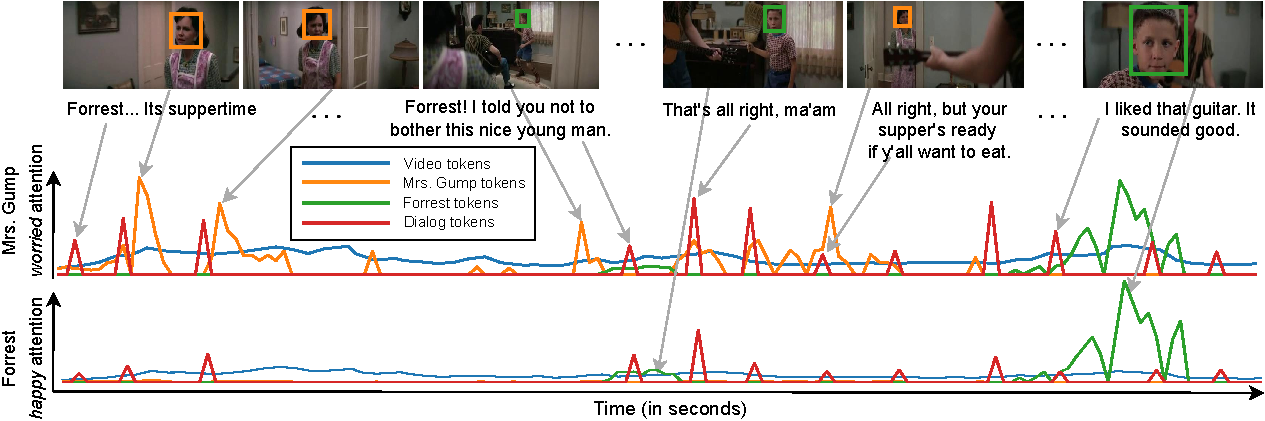
\includegraphics[width=0.99\linewidth]{Figures/qa.pdf}
\vspace{-2mm}
\caption{A scene from the movie \emph{Forrest Gump} showing the multimodal self-attention scores for the two predictions: \emph{Mrs. Gump} is \emph{worried} and \emph{Forrest} is \emph{happy}.
We observe that the \emph{worried} classifier token attends to \emph{Mrs. Gump}'s character tokens when she appears at the start of the scene, while \emph{Forrest}'s \emph{happy} classifier token attends to \emph{Forrest} towards the end of the scene.
The video frames have relatively similar attention scores while dialog helps with emotional utterances such as \emph{told you not to bother} or \emph{it sounded good}.}
\label{fig:qualitative_example}
\end{figure*}

\begin{figure}[t]
\centering
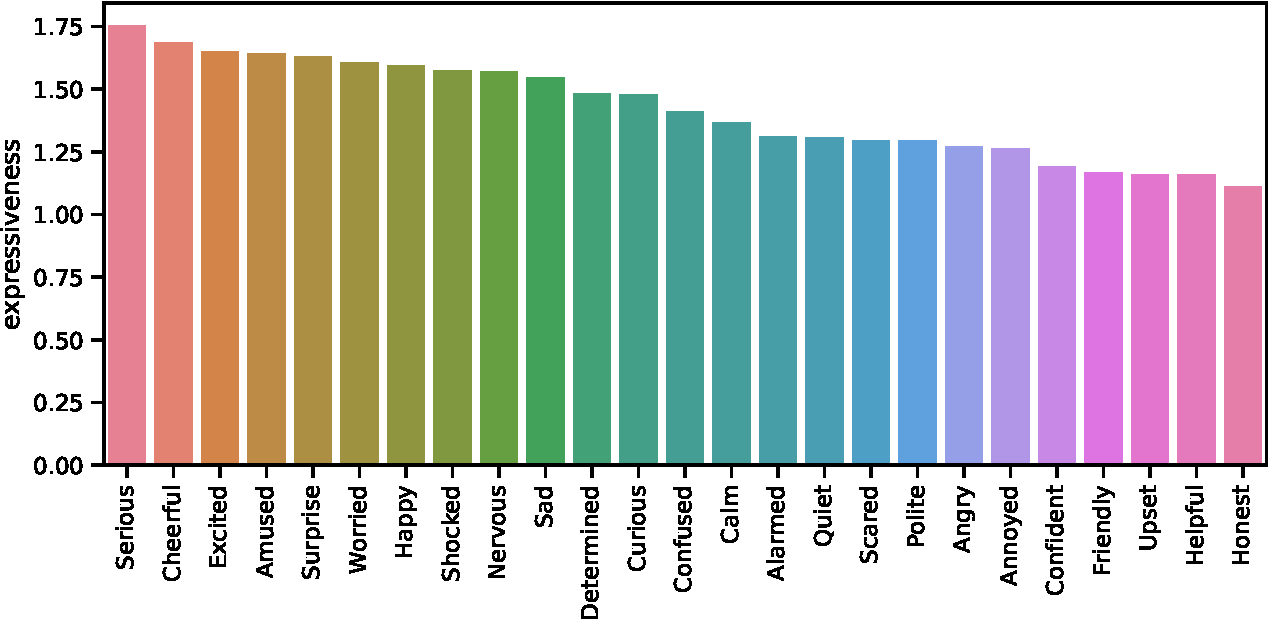
\includegraphics[width=\linewidth]{Figures/expressiveness_25_NEW.pdf}
\vspace{-6mm}
\caption{Sorted expressiveness scores for Top-25 emotions. % on the validation set.
Expressive emotions have higher scores indicating that the model attends to character representations, while mental states have lower scores suggesting more  attention to video and dialog context.}
\label{fig:expression}
\end{figure}

\modelname{} provides an intuitive way to understand which modalities are used to make predictions.
We refer to the self-attention scores matrix as $\alpha$, and analyze specific rows and columns.
Separating the $K$ classifier tokens allows us to find attention-score based evidence for each predicted emotion by looking at a row $\alpha_{\bz_k^{\MS}}$ in the matrix.

Fig.~\ref{fig:qualitative_example} shows an example movie scene where \modelname{} predicts that \emph{Forrest} is \emph{happy} and \emph{Mrs. Gump} is \emph{worried}.
We see that the model pays attention to the appropriate moments and modalities to make the right predictions.

\paragraph{Expressive emotions \vs~Mental states.}
We hypothesize that the self-attention module may focus on character tokens for expressive emotions, while looking at the overall video frames and dialog for the more abstract mental states.
We propose an \emph{expressiveness} score as
\begin{equation}
e_k = \dfrac{ \sum_{i=1}^{N} \sum_{t=1}^{T} \alpha_{\bz_k^{\MS}, \bc_t^i} }
{ \sum_{t=1}^{T} \alpha_{\bz_k^{\MS}, \bbf_t} + \sum_{j=1}^{M} \alpha_{\bz_k^{\MS}, \bu_j} } \, ,
\end{equation}
where $\alpha_{\bz_k^{\MS}, \bc_t^i}$ is the self-attention score between the scene classifier token for emotion $k$ ($\bz_k^{\MS}$) and character $\MP^i$'s appearance in the video frame as $b_t^i$;
$\alpha_{\bz_k^{\MS}, \bbf_t}$ is for the video $f_t$ and
$\alpha_{\bz_k^{\MS}, \bu_j}$ is for dialog utterance $u_j$.
Higher scores indicate expressive emotions as the model focuses on the character features, while lower scores identify mental states that analyze the video and dialog context.
Fig.~\ref{fig:expression} shows the averaged expressiveness score for the Top-25 emotions when the emotion is present in the scene (\ie~$y_k{=}1$).
We observe that mental states such as \emph{honest, helpful, friendly, confident} appear towards the latter half of this plot while most expressive emotions such as \emph{cheerful, excited, serious, surprise} appear in the first half.
Note that the expressiveness scores in our work are for faces and applicable to our particular dataset.
